\documentclass[12pt,landscape]{beamer}
\usepackage[utf8]{inputenc}
\usepackage[czech]{babel}
\usepackage{amsmath}
\usepackage{amsfonts}
\usepackage{amssymb}
\usepackage{graphics}
\usepackage{listings}
\usepackage{array}
\usepackage{hyperref}
\usepackage{tabularx}
\usepackage{booktabs}
\usepackage{caption}
\usepackage{tikz}
\usetheme{Luebeck}
\usecolortheme{seahorse}
%\usecolortheme{lily}

%\definecolor{lightsteel}{RGB}{202,225,255}
\definecolor{SectionBox}{RGB}{60,160,0}

\setbeamertemplate{section in head/foot}{\textcolor{black}{\hfill\textbf{\insertsectionhead}}}
\setbeamertemplate{section in head/foot shaded}{\textcolor{gray}{\hfill\insertsectionhead}}

\setbeamercolor{frametitle}{bg=white}
\setbeamercolor{subsection in head/foot}{bg=white}
%\setbeamercolor{subsection in head/foot}{bg=lightsteel}
%\setbeamertemplate{footline}[frame number]
\setbeamertemplate{footline}
{
        \leavevmode%
        \hbox{%

        \begin{beamercolorbox}[wd=.5\paperwidth,ht=2.5ex,dp=1ex,left]{white}
                \raggedright \usebeamerfont{author in head/foot} ~~\textbf{\insertshorttitle{}}
        \end{beamercolorbox}%
%
        \begin{beamercolorbox}[wd=.4\paperwidth,ht=2.5ex,dp=1ex,right]{section in head/foot}
                \usebeamerfont{title in head/foot}\raggedright ~~\textbf{\insertauthor}
        \end{beamercolorbox}%   

		\begin{beamercolorbox}[wd=.1\paperwidth,ht=2.5ex,dp=1ex,right]{section in head/foot}             
                \raggedleft \textbf{\insertframenumber{} / \inserttotalframenumber}\hspace*{2ex}
        \end{beamercolorbox}}%
%
        \vskip0pt%
}



\captionsetup{labelformat=empty,labelsep=none,justification=justified,width=.75\textwidth,aboveskip=5pt}

%na zacatku sekce obsah
%\AtBeginSection[]
%{
%  \begin{frame}
%    \tableofcontents[currentsection]
%  \end{frame}
%}

\title[Implementace INSPIRE tématu Budovy] % (optional, only for long titles)
{Implementace INSPIRE tématu Budovy}
\subtitle{a rozšiřování XSD schémat\\ ~ \\ 
\includegraphics[scale=0.15]{obrazky/cuzk2.png}}
\author[M.Med] % (optional, for multiple authors)
{Ing. Michal Med}
\date[INSPIRUJME SE... 2015]{INSPIRUJME SE... 2015}

\begin{document}

\begin{frame}[plain]
\titlepage
\end{frame}

\begin{frame}[plain]
\tableofcontents
\end{frame}

\addtobeamertemplate{frametitle}{}{%
\begin{tikzpicture}[remember picture,overlay]
\node[anchor=north east,yshift=2pt,xshift=-10pt] at (current page.north east){
\includegraphics[scale=0.08]{obrazky/cuzk2.png}};
\end{tikzpicture}}


\section{Struktura a obsah datových sad podle INSPIRE}
% Analýza datové specifikace Budovy: aplikační schémata, XSD schémata, Datové sklady, Portrayal

\begin{frame}
\frametitle{INSPIRE}
\begin{center}

\includegraphics[scale=0.45]{obrazky/inspire_logo.png}
\end{center}
\end{frame}

%\begin{frame}
%\frametitle{Standardizace}
%\begin{figure}
%\begin{center}
%
\includegraphics[scale=0.2]{obrazky/inspire_logo.png}~
\includegraphics[scale=0.1]{obrazky/rightarrow.png}~
\includegraphics[scale=0.2]{obrazky/ISO.png}~
\includegraphics[scale=0.1]{obrazky/rightarrow.png}~
\includegraphics[scale=0.1]{obrazky/ogc.jpeg}
%\end{center}
%\end{figure}
%\end{frame}

\begin{frame}
\frametitle{Témata prostorových dat}
\begin{center}
\begin{center}
\begin{tabular}{c c c c c c}

\includegraphics[scale=0.2]{obrazky/INSPIRE_Temata/TN.jpg} & 
\includegraphics[scale=0.2]{obrazky/INSPIRE_Temata/AD.jpg} &

\includegraphics[scale=0.2]{obrazky/INSPIRE_Temata/AM.jpg} & 
\includegraphics[scale=0.2]{obrazky/INSPIRE_Temata/BR.jpg} & 
\includegraphics[scale=0.2]{obrazky/INSPIRE_Temata/BU.jpg} & 
\includegraphics[scale=0.2]{obrazky/INSPIRE_Temata/CP.jpg}\\

\includegraphics[scale=0.2]{obrazky/INSPIRE_Temata/CRS.jpg} & 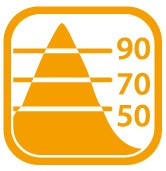
\includegraphics[scale=0.2]{obrazky/INSPIRE_Temata/EL.jpg} &

\includegraphics[scale=0.2]{obrazky/INSPIRE_Temata/SU.jpg} & 
\includegraphics[scale=0.2]{obrazky/INSPIRE_Temata/GE.jpg} & 
\includegraphics[scale=0.2]{obrazky/INSPIRE_Temata/GGS.jpg} & 
\includegraphics[scale=0.2]{obrazky/INSPIRE_Temata/GN.jpg}\\

\includegraphics[scale=0.2]{obrazky/INSPIRE_Temata/HB.jpg} & 
\includegraphics[scale=0.2]{obrazky/INSPIRE_Temata/HH.jpg} &

\includegraphics[scale=0.2]{obrazky/INSPIRE_Temata/HY.jpg} & 
\includegraphics[scale=0.2]{obrazky/INSPIRE_Temata/LC.jpg} & 
\includegraphics[scale=0.2]{obrazky/INSPIRE_Temata/LU.jpg} & 
\includegraphics[scale=0.2]{obrazky/INSPIRE_Temata/MF.jpg}\\

\includegraphics[scale=0.2]{obrazky/INSPIRE_Temata/SD.jpg} & 
\includegraphics[scale=0.2]{obrazky/INSPIRE_Temata/NZ.jpg} &

\includegraphics[scale=0.2]{obrazky/INSPIRE_Temata/SR.jpg} & 
\includegraphics[scale=0.2]{obrazky/INSPIRE_Temata/OI.jpg} & 
\includegraphics[scale=0.2]{obrazky/INSPIRE_Temata/PD.jpg} & 
\includegraphics[scale=0.2]{obrazky/INSPIRE_Temata/PS.jpg}\\
\end{tabular}
\end{center}
\end{center}
\end{frame}

\begin{frame}
\frametitle{Budovy}
\begin{center}

\includegraphics[scale=1]{obrazky/INSPIRE_Temata/BU.jpg}
\end{center}
\end{frame}


\begin{frame}
\frametitle{Aplikační schémata}
\begin{center}
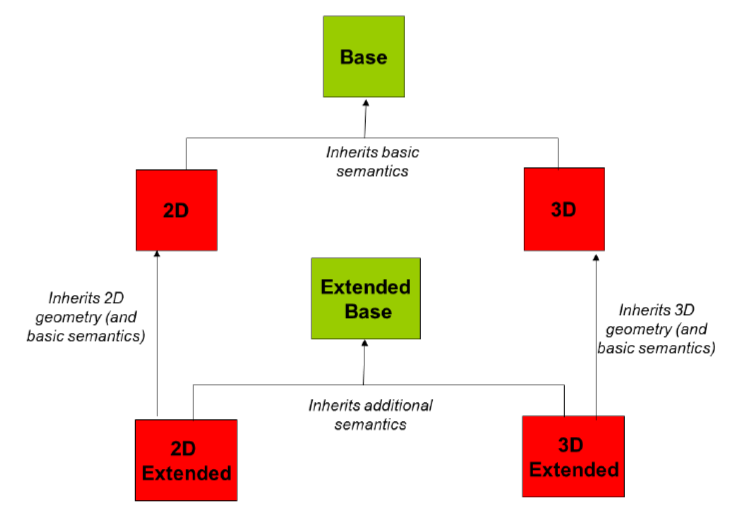
\includegraphics[scale=0.4]{obrazky/app_schema.png}
% celkem šest, dvě abstraktní, čtyři vhodné pro ČR
\end{center}
\end{frame}

\begin{frame}
\frametitle{Schémata XSD}
\begin{itemize}
\item \url{http://www.w3schools.com/schema/}
\end{itemize}
\begin{center}
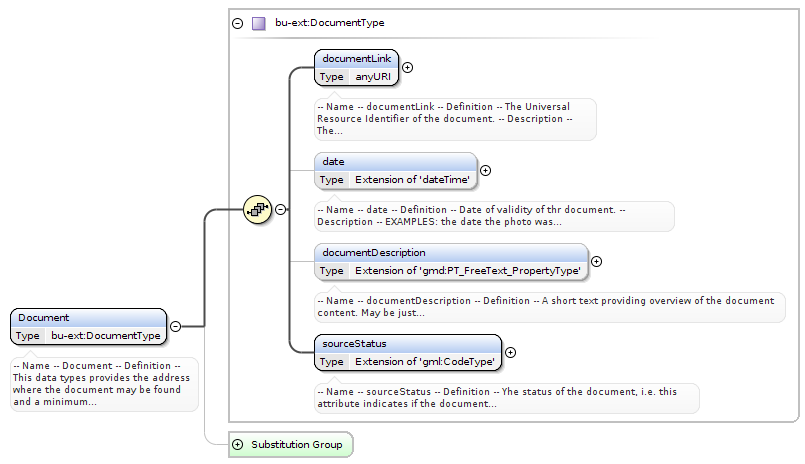
\includegraphics[scale=0.3]{obrazky/XSD.png}
\end{center}
\end{frame}

\begin{frame}
\frametitle{Schémata XSD}
\tiny{
\begin{itemize}
\item \url{http://inspire.ec.europa.eu/schemas/bu-base/3.0/BuildingsBase.xsd}
\item \url{http://inspire.ec.europa.eu/schemas/bu-core2d/3.0/BuildingsCore2D.xsd}
\item \url{http://inspire.ec.europa.eu/schemas/bu-core3d/3.0/BuildingsCore3D.xsd}
\end{itemize}}
\begin{center}

\includegraphics[scale=0.45]{obrazky/missing.jpg}
% pouze tři jsopu zpracované JRC
\end{center}
\end{frame}

\begin{frame}
\frametitle{Rozšiřování aplikačních schémat}
\begin{itemize}
\item Musí vycházet ze stávajících schémat INSPIRE,
\item musí být opatřena dokumentací.
\end{itemize}
\begin{center}
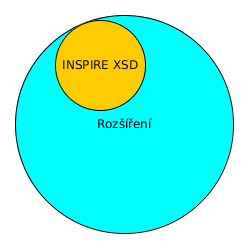
\includegraphics[scale=0.3]{obrazky/extension.png}~
\includegraphics[scale=0.1]{obrazky/rightarrow.png}~
\includegraphics[scale=0.75]{obrazky/data_file.png}
\end{center}
\end{frame}


\begin{frame}
\frametitle{Data INSPIRE}
\begin{itemize}
\item GML 3.2.1 
\end{itemize}
\begin{center}
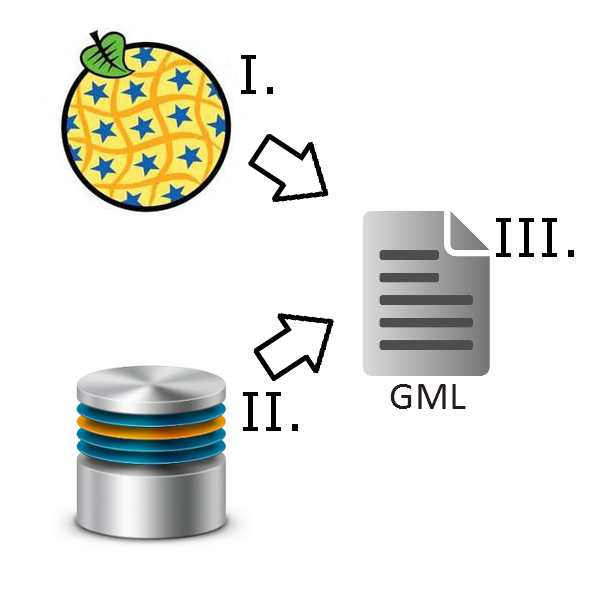
\includegraphics[scale=0.35]{obrazky/data_tvorba.png}
\end{center}
\end{frame}

\begin{frame}
\frametitle{Zdroje dat}
\begin{center}
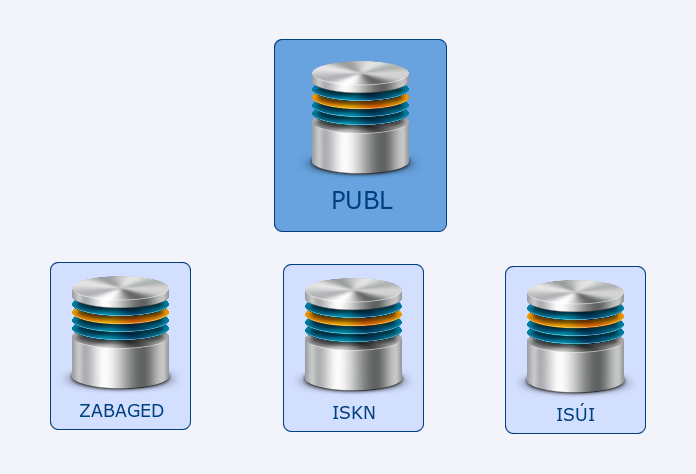
\includegraphics[scale=0.4]{obrazky/data_source.png}
\end{center}
\end{frame}

\begin{frame}
\frametitle{Poskytování a vzhled}
\begin{center}
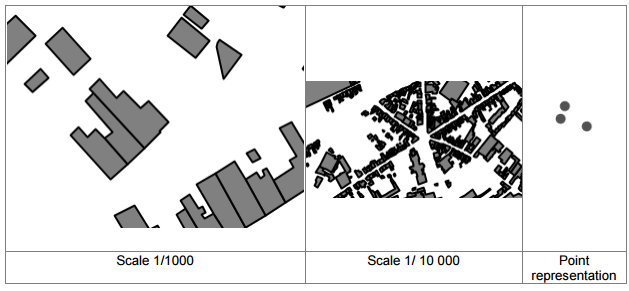
\includegraphics[scale=0.45]{obrazky/portrayal_bu.png}
\end{center}
\end{frame}

\begin{frame}
\frametitle{Poskytování a vzhled}
\begin{center}
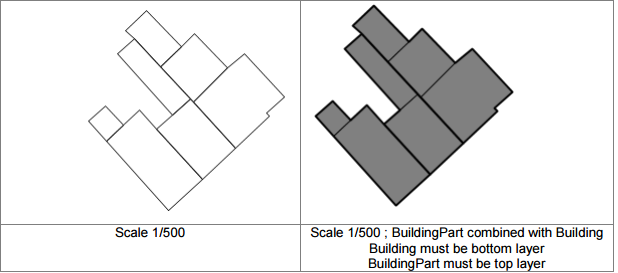
\includegraphics[scale=0.45]{obrazky/portrayal_bp.png}
\end{center}
%více v poslední kapitole
\end{frame}% Analýza datové specifikace Budovy: aplikační schémata, XSD schémata, Datové sklady, Portrayal

\section{Tvorba a rozšiřování schémat XSD}
% Jaká aplikační schémata pro BU jsou implementovaná do XSD 

\begin{frame}
\frametitle{Aplikační schémata tématu Budovy}
\begin{center}
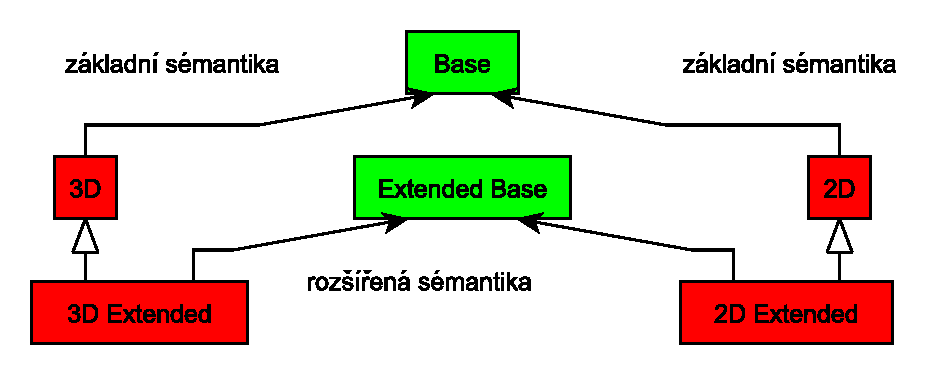
\includegraphics[scale=0.7]{obrazky/BU_schemas.pdf}
\end{center}
\end{frame}

\begin{frame}
\frametitle{Možnosti implementace aplikačních schémat}
\begin{center}
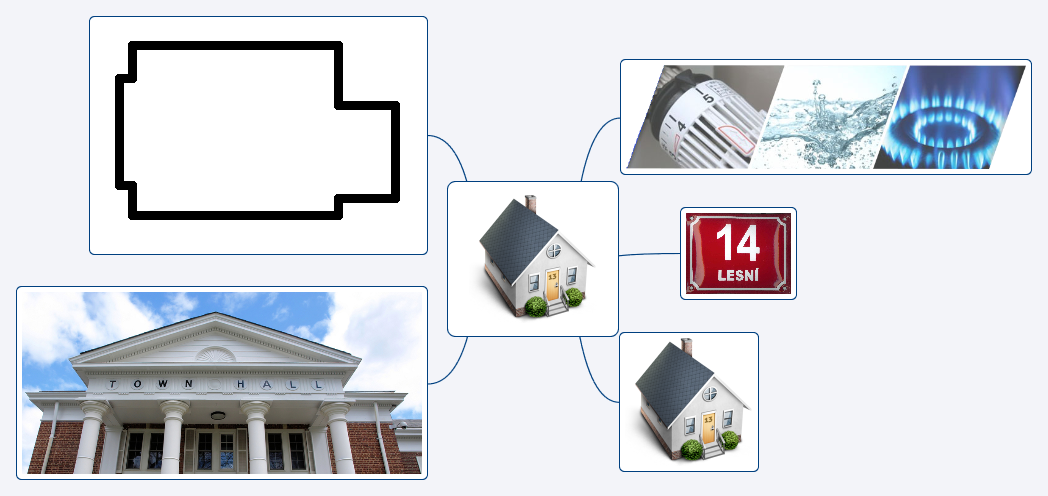
\includegraphics[scale=0.3]{obrazky/connection.png}
\end{center}
\end{frame}

\begin{frame}
\frametitle{Tvorba XSD -- základ}
\begin{center}
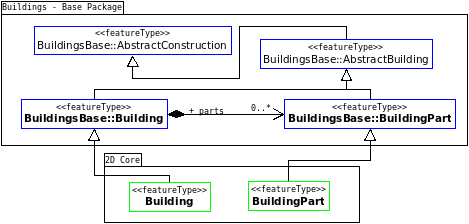
\includegraphics[scale=0.65]{obrazky/BuildingsBase2D.png}
\end{center}
\end{frame}

\begin{frame}
\frametitle{Tvorba XSD -- dědičnost}
\begin{center}
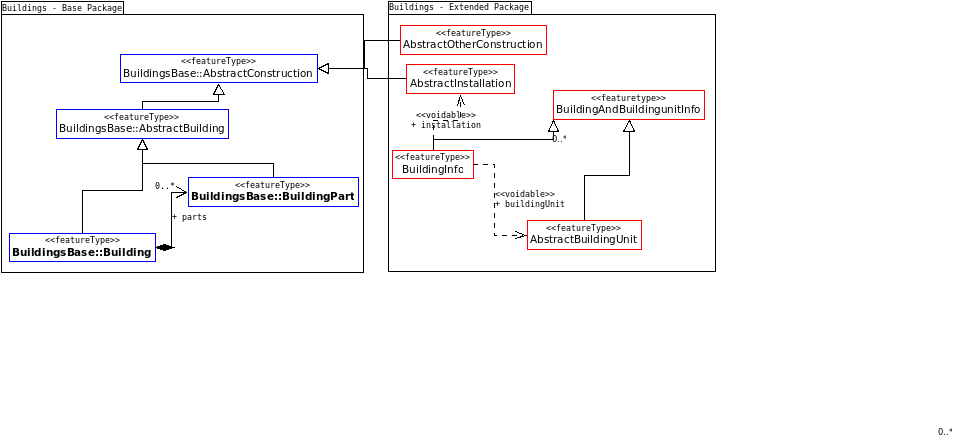
\includegraphics[scale=0.45]{obrazky/BU_ExtDedicnost.png}
\end{center}
\end{frame}

\begin{frame}
\frametitle{Tvorba XSD -- dědičnost}
\begin{center}
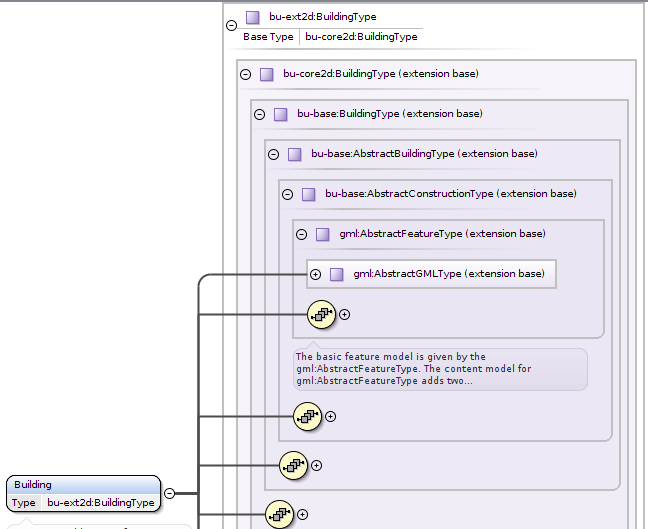
\includegraphics[scale=0.35]{obrazky/BU_oXygen.png}
\end{center}
\end{frame}

\begin{frame}
\frametitle{Tvorba XSD -- geometrie}
\begin{center}
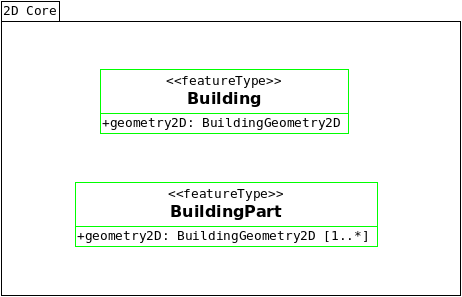
\includegraphics[scale=0.45]{obrazky/geometrie.png}
\end{center}
\end{frame}

\begin{frame}
\frametitle{Tvorba XSD -- vícenásobná dědičnost}
\begin{center}
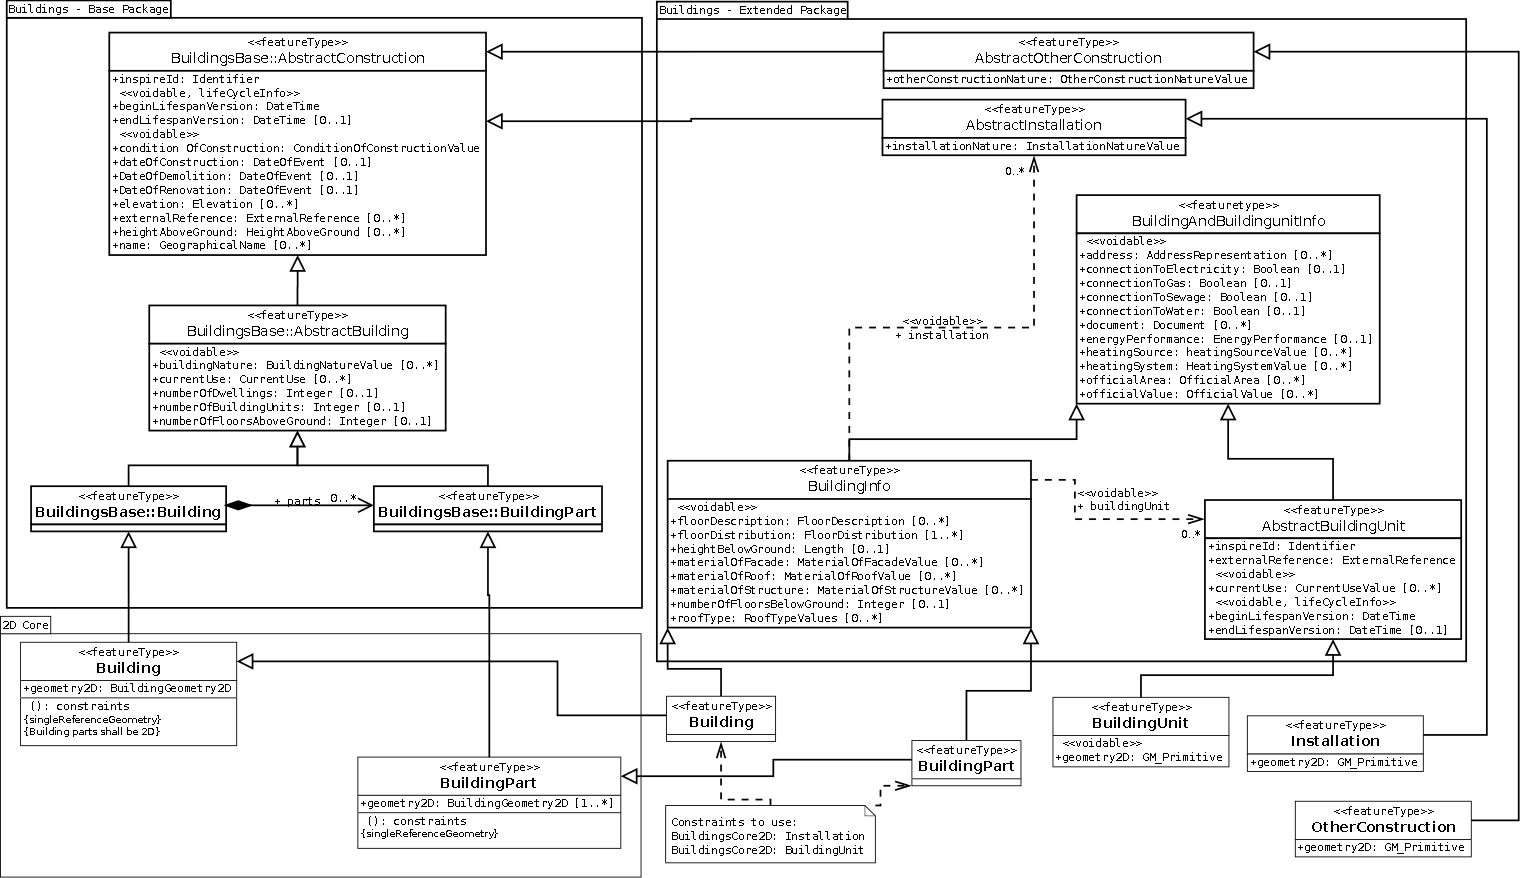
\includegraphics[scale=0.15]{obrazky/BuildingsExtended2D.png}
\end{center}
\end{frame}

\begin{frame}
\frametitle{Tvorba XSD -- vícenásobná dědičnosti}
\begin{center}
\includegraphics[scale=0.4]{obrazky/BU_dedicnost_info.png}
\end{center}
\end{frame}

\begin{frame}
\frametitle{Nová schémata XSD}
\begin{itemize}
\item \url{http://services.cuzk.cz/xsd/inspire/bu-ext2d/3.0/BuildingsExtended2D.xsd}
\item \url{http://services.cuzk.cz/xsd/inspire/bu-ext/3.0/BuildingsExtendedBase.xsd}
\end{itemize}
\end{frame}

% Tvorba XSD schémata pro Budovy

\section{Implementace a publikace}
% Přístup k datům, WMS, WFS, předpřipravené soubory

%\begin{frame}
%\frametitle{Původ dat}
%\begin{center}
%\includegraphics[scale=0.65]{obrazky/various_buildings_possibilities.png}
%\end{center}
%\end{frame}

%\begin{frame}
%\frametitle{Transformace dat}
%\begin{center}
%\includegraphics[scale=0.45]{obrazky/transformace.png}
%\end{center}
%\end{frame}

%\begin{frame}
%\frametitle{Publikační databáze -- tabulky}
%\begin{center}
%\includegraphics[scale=0.26]{obrazky/BU_PUBL_DB.png}
%\end{center}
%\end{frame}

\begin{frame}
\frametitle{Publikační databáze -- pohledy}
\begin{center}
\includegraphics[scale=0.12]{obrazky/pohled.jpg}
\end{center}
\end{frame}

\begin{frame}
\frametitle{Vzorový GML soubor}
\begin{center}
\includegraphics[scale=0.3]{obrazky/GML_sablona.png}
\end{center}
\end{frame}

\begin{frame}
\frametitle{Přístup k datům}
\begin{center}
\includegraphics[scale=0.5]{obrazky/distribuce.png}
\end{center}
\end{frame}

\begin{frame}
\frametitle{Prohlížecí služby -- Building}
\begin{center}
tady bude obrázek wms
\end{center}
\end{frame}

\begin{frame}
\frametitle{Prohlížecí služby -- BuildingPart}
\begin{center}
tady bude obrázek wms
\end{center}
\end{frame}

\begin{frame}
\frametitle{Stahovací služby}
\begin{center}
tady bude obrázek wfs vizualizovaný v QGIS
\end{center}
\end{frame}

\begin{frame}
\frametitle{Předpřipravené GML}
\begin{center}
tady bude obrázek ukazující distribuci pomocí ATOM, WFS nebo vystavením na webu
\end{center}
\end{frame}% Přístup k datům, WMS, WFS, předpřipravené soubory

\frame[plain]{
\huge{Díky za pozornost}
\begin{center}
\includegraphics[scale=0.6]{obrazky/otazky}
\end{center}
}

\end{document}